\section{mr::simple\_\-timer Class Reference}
\label{classmr_1_1simple__timer}\index{mr::simple_timer@{mr::simple\_\-timer}}
{\tt \#include $<$mr\-Profile.h$>$}

Inheritance diagram for mr::simple\_\-timer::\begin{figure}[H]
\begin{center}
\leavevmode
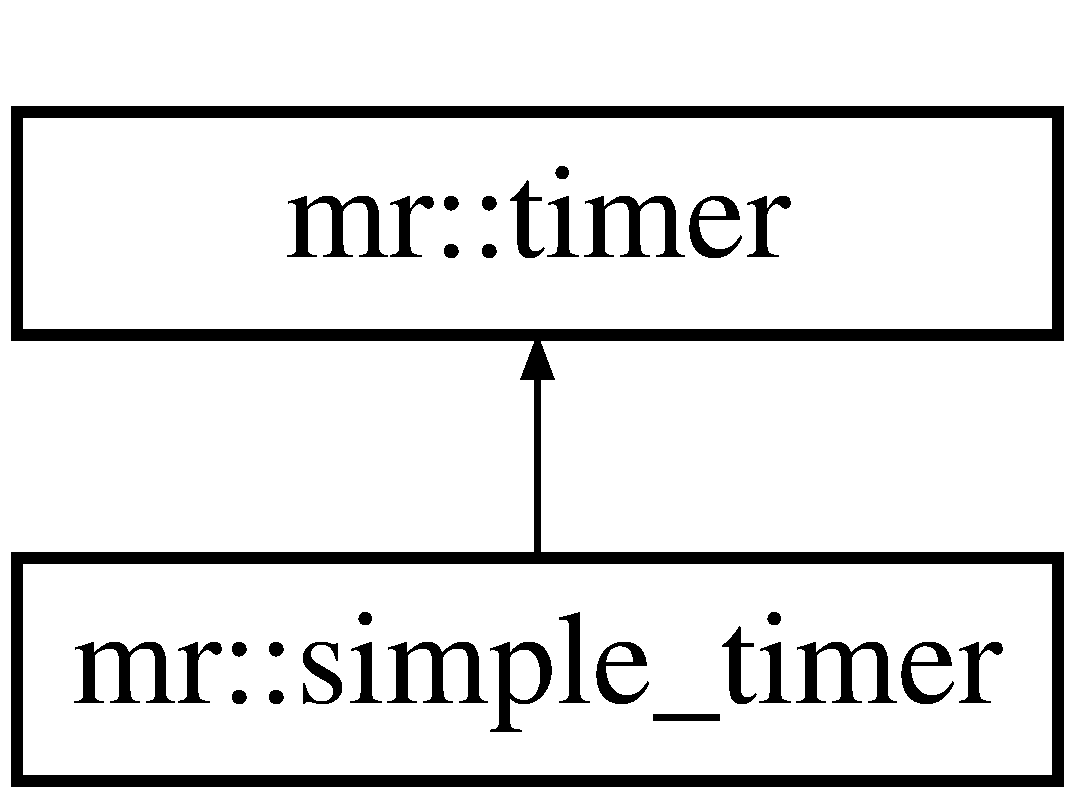
\includegraphics[height=2cm]{classmr_1_1simple__timer}
\end{center}
\end{figure}


\subsection{Detailed Description}
Very simple class/macro for profiling stuff... Just use MR\_\-TIME\_\-IT macro and enclose area in \{\}, like...



\footnotesize\begin{verbatim}      {
        MR_TIME_IT;
         ....stuff to profile...
      }  // here it will print result
\end{verbatim}
\normalsize




The documentation for this class was generated from the following file:\begin{CompactItemize}
\item 
{\bf mr\-Profile.h}\end{CompactItemize}
